%
% Copyright (c) 2013 The NetBSD Foundation, Inc.
% All rights reserved.
%
% This code is derived from software contributed to The NetBSD Foundation
% by Radoslaw Kujawa.
%
% Redistribution and use in source and binary forms, with or without
% modification, are permitted provided that the following conditions
% are met:
% 1. Redistributions of source code must retain the above copyright
%    notice, this list of conditions and the following disclaimer.
% 2. Redistributions in binary form must reproduce the above copyright
%    notice, this list of conditions and the following disclaimer in the
%    documentation and/or other materials provided with the distribution.
%
% THIS SOFTWARE IS PROVIDED BY THE NETBSD FOUNDATION, INC. AND CONTRIBUTORS
% ``AS IS'' AND ANY EXPRESS OR IMPLIED WARRANTIES, INCLUDING, BUT NOT LIMITED
% TO, THE IMPLIED WARRANTIES OF MERCHANTABILITY AND FITNESS FOR A PARTICULAR
% PURPOSE ARE DISCLAIMED.  IN NO EVENT SHALL THE FOUNDATION OR CONTRIBUTORS
% BE LIABLE FOR ANY DIRECT, INDIRECT, INCIDENTAL, SPECIAL, EXEMPLARY, OR
% CONSEQUENTIAL DAMAGES (INCLUDING, BUT NOT LIMITED TO, PROCUREMENT OF
% SUBSTITUTE GOODS OR SERVICES; LOSS OF USE, DATA, OR PROFITS; OR BUSINESS
% INTERRUPTION) HOWEVER CAUSED AND ON ANY THEORY OF LIABILITY, WHETHER IN
% CONTRACT, STRICT LIABILITY, OR TORT (INCLUDING NEGLIGENCE OR OTHERWISE)
% ARISING IN ANY WAY OUT OF THE USE OF THIS SOFTWARE, EVEN IF ADVISED OF THE
% POSSIBILITY OF SUCH DAMAGE.
%
% 
\documentclass[dvipsnames,table]{beamer}
\usepackage{polski}

\usetheme{Rochester}
\usecolortheme{orchid}

\usepackage{listings}
\usepackage{ucs}
\usepackage[utf8x]{inputenc}
\usepackage{wasysym}
\usepackage[normalem]{ulem}
\usepackage{amsmath}
\usepackage{hyperref}

\setbeamertemplate{navigation symbols}{}
\setbeamertemplate{caption}[numbered]
\setbeamerfont{caption}{size=\scriptsize}
\setbeamercolor{framenote}{bg=NetBSD-orange!25}
\setbeamercolor{rednote}{bg=Red!25}
\setbeamercolor{palette primary}{use=structure,fg=white,bg=NetBSD-orange}
\setbeamercolor{palette secondary}{use=structure,fg=white,bg=NetBSD-orange2}

\setbeamertemplate{itemize item}{\scriptsize\raise1pt\hbox{\donotcoloroutermaths$\blacktriangleright$}}
\setbeamertemplate{itemize subitem}{\tiny\raise1pt\hbox{\donotcoloroutermaths$\bullet$}}
\setbeamertemplate{itemize subsubitem}{\tiny\raise1pt\hbox{\donotcoloroutermaths{--}}}

\setbeamertemplate{enumerate item}{\insertenumlabel.}
\setbeamertemplate{enumerate subitem}{\insertenumlabel.\insertsubenumlabel}
\setbeamertemplate{enumerate subsubitem}{\insertenumlabel.\insertsubenumlabel.\insertsubsubenumlabel}
\setbeamertemplate{enumerate mini template}{\insertenumlabel}

\setbeamercolor{itemize item}{fg=NetBSD-orange, bg=NetBSD-orange}
\setbeamercolor{itemize subitem}{fg=NetBSD-orange, bg=NetBSD-orange}
\setbeamercolor{itemize subsubitem}{fg=NetBSD-orange, bg=NetBSD-orange}

\setbeamercolor{section number projected}{fg=white,bg=NetBSD-orange}
\setbeamercolor{subsection number projected}{fg=white,bg=NetBSD-orange}
\setbeamercolor{button}{bg=NetBSD-orange,fg=white}

\setbeamertemplate{section in toc}[circle]
\setbeamertemplate{subsection in toc}[square]


\definecolor{NetBSD-orange}{RGB}{242,103,17}
\definecolor{NetBSD-orange2}{RGB}{177,76,12}
\hypersetup{colorlinks=true,linkcolor=white,urlcolor=NetBSD-orange}

\setlength{\tabcolsep}{8pt}
\renewcommand{\arraystretch}{1.2}

\newcommand{\nbsdcolor}[1] {
	{\color{NetBSD-orange} #1}
}

\lstset{
   language=sh,
   basicstyle=\tiny,
   breaklines=true,
   escapechar=\@,
   commentstyle=\color{NetBSD-orange}
}

\AtBeginSection[]{
\frame{

\begin{center}

{\usebeamerfont{section name}\usebeamercolor[fg]{section name}Część~\insertsectionnumber}
    \vskip1em\par

	\begin{beamercolorbox}[sep=12pt,center]{palette primary}
		\usebeamerfont{section title}\insertsection\par
	\end{beamercolorbox}
\end{center}

%\sectionpage
}
}

\title{System operacyjny NetBSD\\ w zastosowaniach wbudowanych}


\author{Radoslaw Kujawa -- rkujawa@NetBSD.org}

\institute{The NetBSD Foundation / OSEC}

\begin{document}

\begin{frame}
\titlepage
\end{frame}

\begin{frame}[allowframebreaks]
\frametitle{Spis treści}
{
\hypersetup{colorlinks=true,linkcolor=black,urlcolor=NetBSD-orange}
\tableofcontents
}
\end{frame}

\section{Garść informacji na temat NetBSD}

\begin{frame}
\frametitle{Czym jest NetBSD?}
\begin{itemize}
	\item UNIX-owy system operacyjny
	\item Nie tylko jądro, ale \textbf{kompletny} system operacyjny
	\item Dostarcza także interfejs graficzny (X Window System)
	\item Oprogramowanie producentów trzecich dostępne poprzez pkgsrc (ponad 12000 paczek)
\end{itemize}
\end{frame}

\begin{frame}
\frametitle{Historia NetBSD w pigułce}
\begin{itemize}
	\item Projekt NetBSD istnieje od 20 lat
	\item Wywodzi się z Berkeley Software Distribution -- systemu operacyjnego rozwijanego w grupie CSRG na Uniwersytecie w Berkeley, Kalifornia
	\item Korzenie systemu sięgają kodu oryginalnego UNIXa (1969) -- prawie pół wieku historii
\end{itemize}
\end{frame}

\begin{frame}
\frametitle{Cechy NetBSD}
\begin{itemize}
	\item Małe wymagania sprzętowe (ok. 24MB RAM, 300MB przestrzeni masowej)
	\item Bardzo dobra przenośność -- 57 platform, 12 architektur CPU
	\item Przykładanie uwagi do ,,czystości'' projektu oraz implementacji
	\item W zgodzie z duchem UNIXa
	\item Kompletna dokumentacja interfejsów programistycznych
	\item Ostrożne podejście do nowinek
	\item Niski ,,próg wejścia'' dla nowych programistów
	\item Powyższe cechy czynią NetBSD doskonałym systemem operacyjnym dla:
	\begin{itemize}
		\item \textbf{Rozwiązań wbudowanych}
		\item Prac badawczych nad nowymi technologiami w informatyce
		\item Serwerów (w niektórych zastosowaniach)
		\item Komputerów osobistych o małej mocy obliczeniowej
	\end{itemize}
	\item Licencja BSD przyjazna komercyjnemu wykorzystaniu
\end{itemize}
\end{frame}

\begin{frame}
\frametitle{Cechy systemu wbudowanego}
\begin{itemize}
	\item Antyteza systemu ogólnego przeznaczenia
	\item Pełni ściśle określone przez twórców funkcje
	\item Ograniczone możliwości dostosowania i konfiguracji
	\item Sprzęt oraz oprogramowanie zwykle mocno zintegrowane
	\item Wysoka niezawodność
	\item Typowe systemy wbudowane: dekodery TV, telewizory, lodówki, komputery w samochodach, urządzenia sieciowe (routery, switche), sprzęt pomiarowy, systemy alarmowe
	\item Powoli zaciera się granica między sprzętem wykorzystywanym w systemach wbudowanych a komputerach ogólnego przeznaczenia
\end{itemize}
\end{frame}

\begin{frame}
\frametitle{Wykorzystanie i rozwój NetBSD}
\begin{itemize}
\item Kto używa NetBSD?
\begin{itemize}
	\item Powszechnie znane firmy oraz organizacje
	\begin{itemize}
		\item Apple - AirPort Extreme, Time Capsule, różne komponenty OS X oraz iOS
		\item Blackberry/RIM - Stos IP, sterowniki, pkgsrc w systemie QNX
		\item Dell - \href{http://www.dell.com/us/business/p/force10-ftos/pd}{Force10 OS}
 		\item Microsoft - Architektura \href{http://research.microsoft.com/en-us/projects/emips/}{eMIPS}
		\item micro systems - Kasy fiskalne, POSy \href{http://www.arcapos.ch/produkt/}{arcapos}
		\item NASA - International Space Station
		\item oraz inni
	\end{itemize}
	\item Hobbyści i hakerzy
	\item Naukowcy i uniwersytety
\end{itemize}
\item{Kto pracuje nad NetBSD?}
\begin{itemize}
	\item Niezależni developerzy zrzeszeni w fundacji NetBSD
	\item Firmy - w ramach projektów lub kontraktów (np. Semihalf, 3am Software Foundry, Genetec, inni)
\end{itemize}

\end{itemize}
\end{frame}


\begin{frame}
\frametitle{Jądro NetBSD}
\begin{itemize}
	\item Klasyczne jądro monolityczne z modułami\footnote{Systemy wbudowanie zwykle nie wykorzystują modułów.}
	\item Oferuje ochronę pamięci i pamięć wirtualną -- wymaga jednostki zarządzania pamięcią (MMU)
	\item Napisane w C, z małymi wstawkami w asemblerze
	\item Większość kodu niezależna od platformy sprzętowej
	\item Mechanizmy ułatwiające pisanie kodu zależnego od platformy oraz sterowników urządzeń
	\begin{itemize}
		\item \href{http://netbsd.gw.com/cgi-bin/man-cgi?bus_space++NetBSD-current}{bus\_space(4)}, \href{http://netbsd.gw.com/cgi-bin/man-cgi?bus_dma++NetBSD-current}{bus\_dma(4)}
		\item Autokonfiguracja
	\end{itemize}
	\item Wbudowany w jądro debugger
\end{itemize}
\end{frame}


\begin{frame}
\frametitle{Jądro NetBSD -- autokonfiguracja}
\begin{center}
	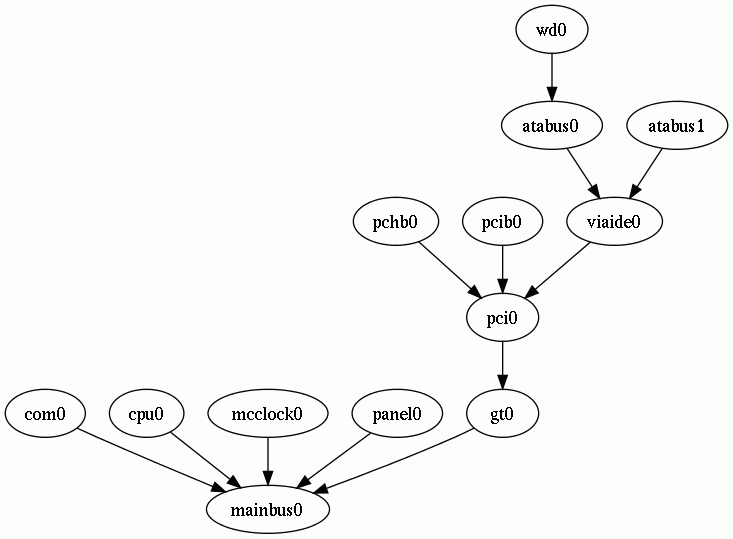
\includegraphics[scale=0.4]{img_cobaltdmesg.png}
\end{center}
\end{frame}

\begin{frame}
\frametitle{Budowanie NetBSD ze źródeł}
\begin{itemize}
	\item Procedura budowania systemu ze źródeł jest trywialna
	\begin{itemize}
		\item Ściągnięcie kodu źródłowego NetBSD
		\item \tt{./build.sh -m [port] tools}
		\item \tt{./build.sh -m [port] distribution}
	\end{itemize}
	\item Skrypt build.sh jest tylko opakowauje standardowe pliki Makefile
	\item Kompilacja wskrośna całego systemu możliwa z prawie każdego innego systemu UNIX-owego (Linux, MacOS X, *BSD, Solaris, itd.), także o innej architekturze procesora
\end{itemize}
\end{frame}


\section{Budowa aplikacji wbudowanych na NetBSD}

\begin{frame}
\frametitle{Od czego zacząć?}
\begin{itemize}
	\item Pomysł -- patrz poprzedni wykład {\Large \smiley}
	\item Wybór zestawu ewaluacyjnego (platformy sprzętowej)
	\item Wybór lub wytworzenie dodatkowych modułów sprzętowych
	\item Implementacja oprogramowania
	\item Jeśli produkcja masowa: projekt i budowa własnego sprzętu
\end{itemize}
\end{frame}	

\begin{frame}
\frametitle{Wybór platformy sprzętowej}
\begin{itemize}
	\item Czy architektura procesora (powerpc, arm, mips, ...) jest już obsługiwana? 
	\item Czy platforma sprzetowa, którą chcę wykorzystać jest już obsługiwana?
	\item Czy wszystkie peryferia są obsługiwane?
	\item Słowo ,,port'' w terminologii NetBSD
	\item Dzięki modularnej architekturze NetBSD przeniesienie (,,portowanie'') systemu na nową platformę, czy dodanie wsparcia dla nowego typu procesora jest wzlgędnie proste
\end{itemize}
\end{frame}

\begin{frame}
\frametitle{Dostęp do sprzętu w aplikacji wbudowanej}
\begin{itemize}
	\item W systemach opartych na 8-bitowych oraz 16-bitowych mikrokontrolerach zwyczajem jest bezpośredni dostęp do sprzętu
	\item NetBSD jako tradycyjny system UNIX-owy implementuje ochronę pamięci i pamięć wirtualną
	\begin{itemize}
		\item Ściśle zdefiniowany interfejs między jądrem a przestrzenią użytkownika
		\item Większa niezawodność i bezpieczeństwo
	\end{itemize}
\end{itemize}
\begin{center}
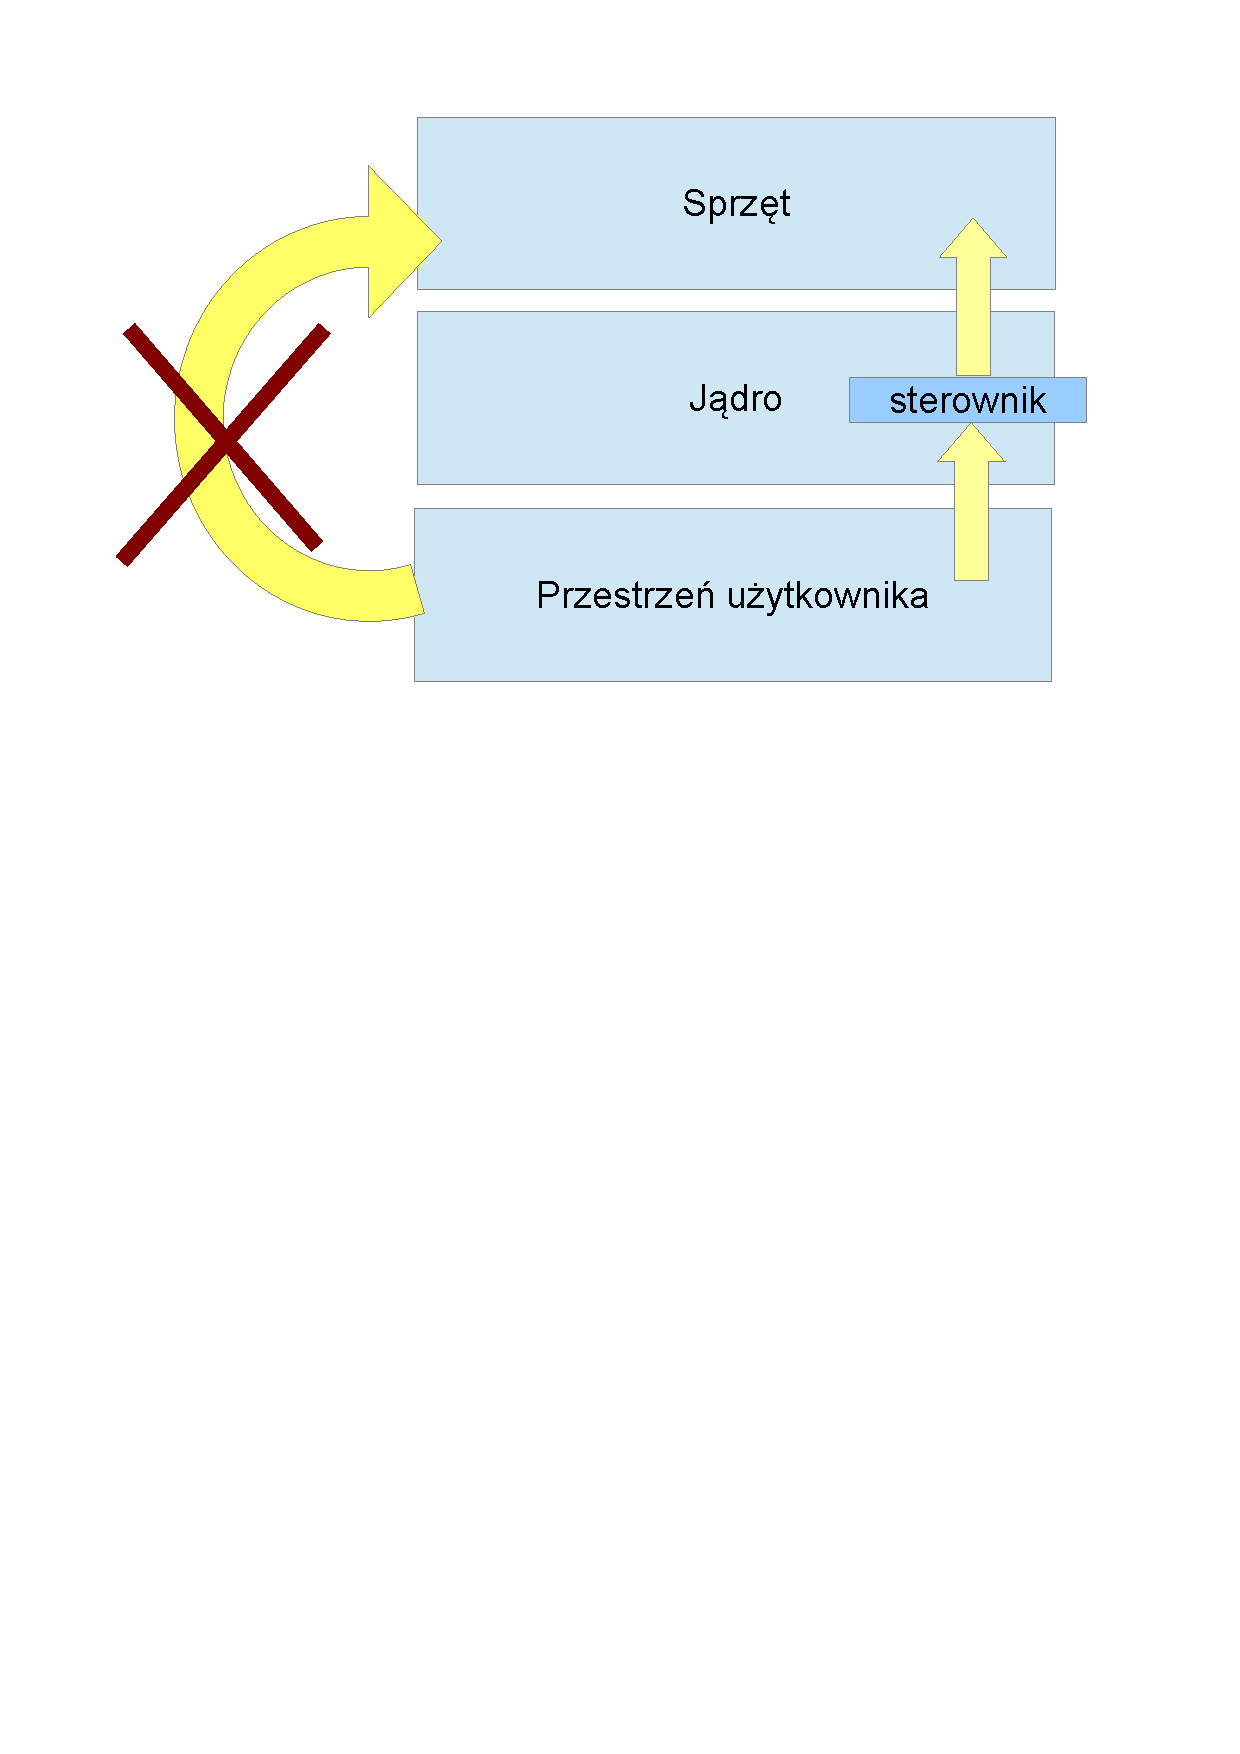
\includegraphics[scale=0.33]{img_hwaccess.pdf}
\end{center}
\end{frame}

\begin{frame}
\frametitle{Aplikacja wbudowana w przestrzeni użytkownika}
\begin{itemize}
	\item Aplikacja wbudowana jest zwykłym programem działającym w przestrzeni użytkownika
	\item Programista znający rozwiązania open source czuje się ,,jak w domu''
	\item Standardy API: ANSI C, POSIX, inne typowe dla UNIXa
	\item Wiele bibliotek w komplecie -- nie ma potrzeby wynajdywania koła na nowo
	\item Potrzebna dodatkowa funkcjonalność? pkgsrc
	\item Brak wymagań dot. działania innych procesów -- aplikacja może zastąpić init'a
\end{itemize}
\end{frame}

\begin{frame}
\frametitle{Konfiguracja jądra w systemie wbudowanym}
\begin{itemize}
	\item Jądro zbudowane bez modułów
	\item Plik konfiguracyjny jądra opisuje jakie funkcjonalności oraz jakie sterowniki mają być skompilowane w danym jądrze
	\item W systemach wbudowanych opartych o NetBSD plik konfiguracyjny jądra określa też pod jakimi adresami znajdują się peryferia
	\item ...
	\item W Linux i FreeBSD przyjęto inne rozwiązanie do tego samego celu - Flattened Device Tree
\end{itemize}
\end{frame}




\begin{frame}
\frametitle{Sprzęt do rozwoju aplikacji wbudowanych}
\begin{itemize}
	\item Łatwo dostępne zestawy uruchomieniowe i ewaluacyjne
	\begin{itemize}
		\item Raspberry Pi
		\item Beagleboard, Beaglebone
		\item Pandaboard
		\item wiele innych

	\end{itemize}
	\item Możliwość wykorzystania niektórych produktów ,,z półki'' jako zestawu
	\begin{itemize}
		\item NAS oparte o PowerPC MPC824x - znane produkty firm Synology, QNAP (sandpoint)
		\item Linksys NSLU2 (evbarm)
		\item Nokia N900 (evbarm)
		\item oraz inne
	\end{itemize}
\end{itemize}
\end{frame}

\section{Prosta aplikacja wbudowana}

\begin{frame}
\frametitle{Beaglebone}

\begin{columns}[c]
\column{3in}

\begin{itemize}

	\item SoC Texas Instruments AM335x 720MHz
	\item 32-bitowa architektura ARM v7
	\item 256MB DDR2 SDRAM
	\item Slot micro SD, Ethernet, host USB
	\item Ustandaryzowane złącza pozwalają na dołączanie dodatkowych modułów (,,cape'' jak ,,shield'' w Arduino)
	\item Interfejsy typowe dla mikrokontrolerów - SPI, I\textsuperscript{2}C, ADC, CAN, itd.
	\item Teraz dostępna nowa wersja ,,Black'' - 1GHz, 512MB DDR3, HDMI (\$45)
\end{itemize}

\column{1.5in}
	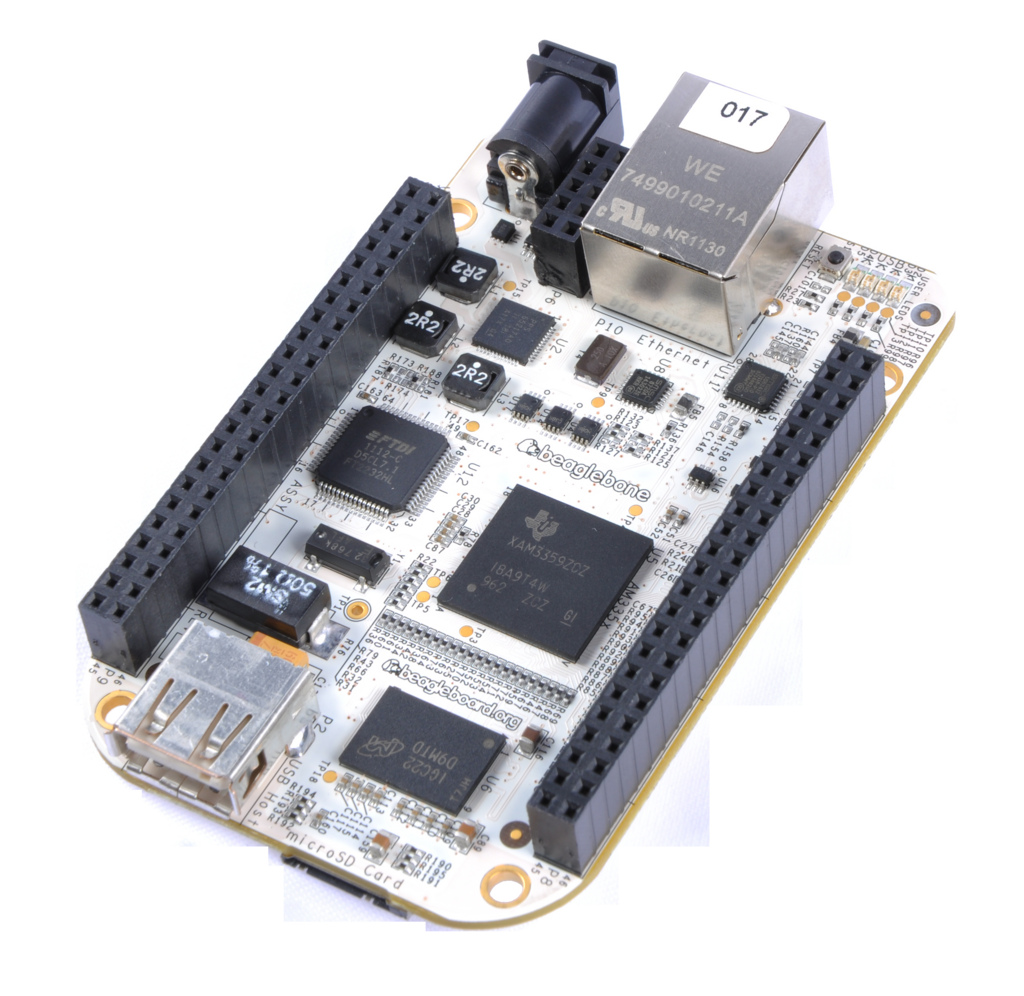
\includegraphics[scale=0.5]{img_beaglebone.jpg}
\end{columns}
\end{frame}

\begin{frame}
\frametitle{Aplikacja wbudowana -- założenia funkcjonalne}
\begin{itemize}
	\item System wbudowany -- monitoring regulacji napięcia
	\item Odczyt obecnego stanu regulatorów dostępnych na BeagleBone
	\item Webowy interfejs użytkownika pozwalający na przedstawienie obecnego stanu regulatorów
\end{itemize}
\end{frame}


\begin{frame}
\frametitle{Aplikacja wbudowna -- peryferia}
\begin{itemize}
	\item Texas Instruments \href{http://www.ti.com/product/tps65217b}{TPS65217B}
	\item Interfejs - szyna I\textsuperscript{2}C, adres 0x24
	\item Napięcie wejściowe 5V (USB, zasilacz lub bateria)
	\item 7 niezależnych regulatorów napięcia
\end{itemize}
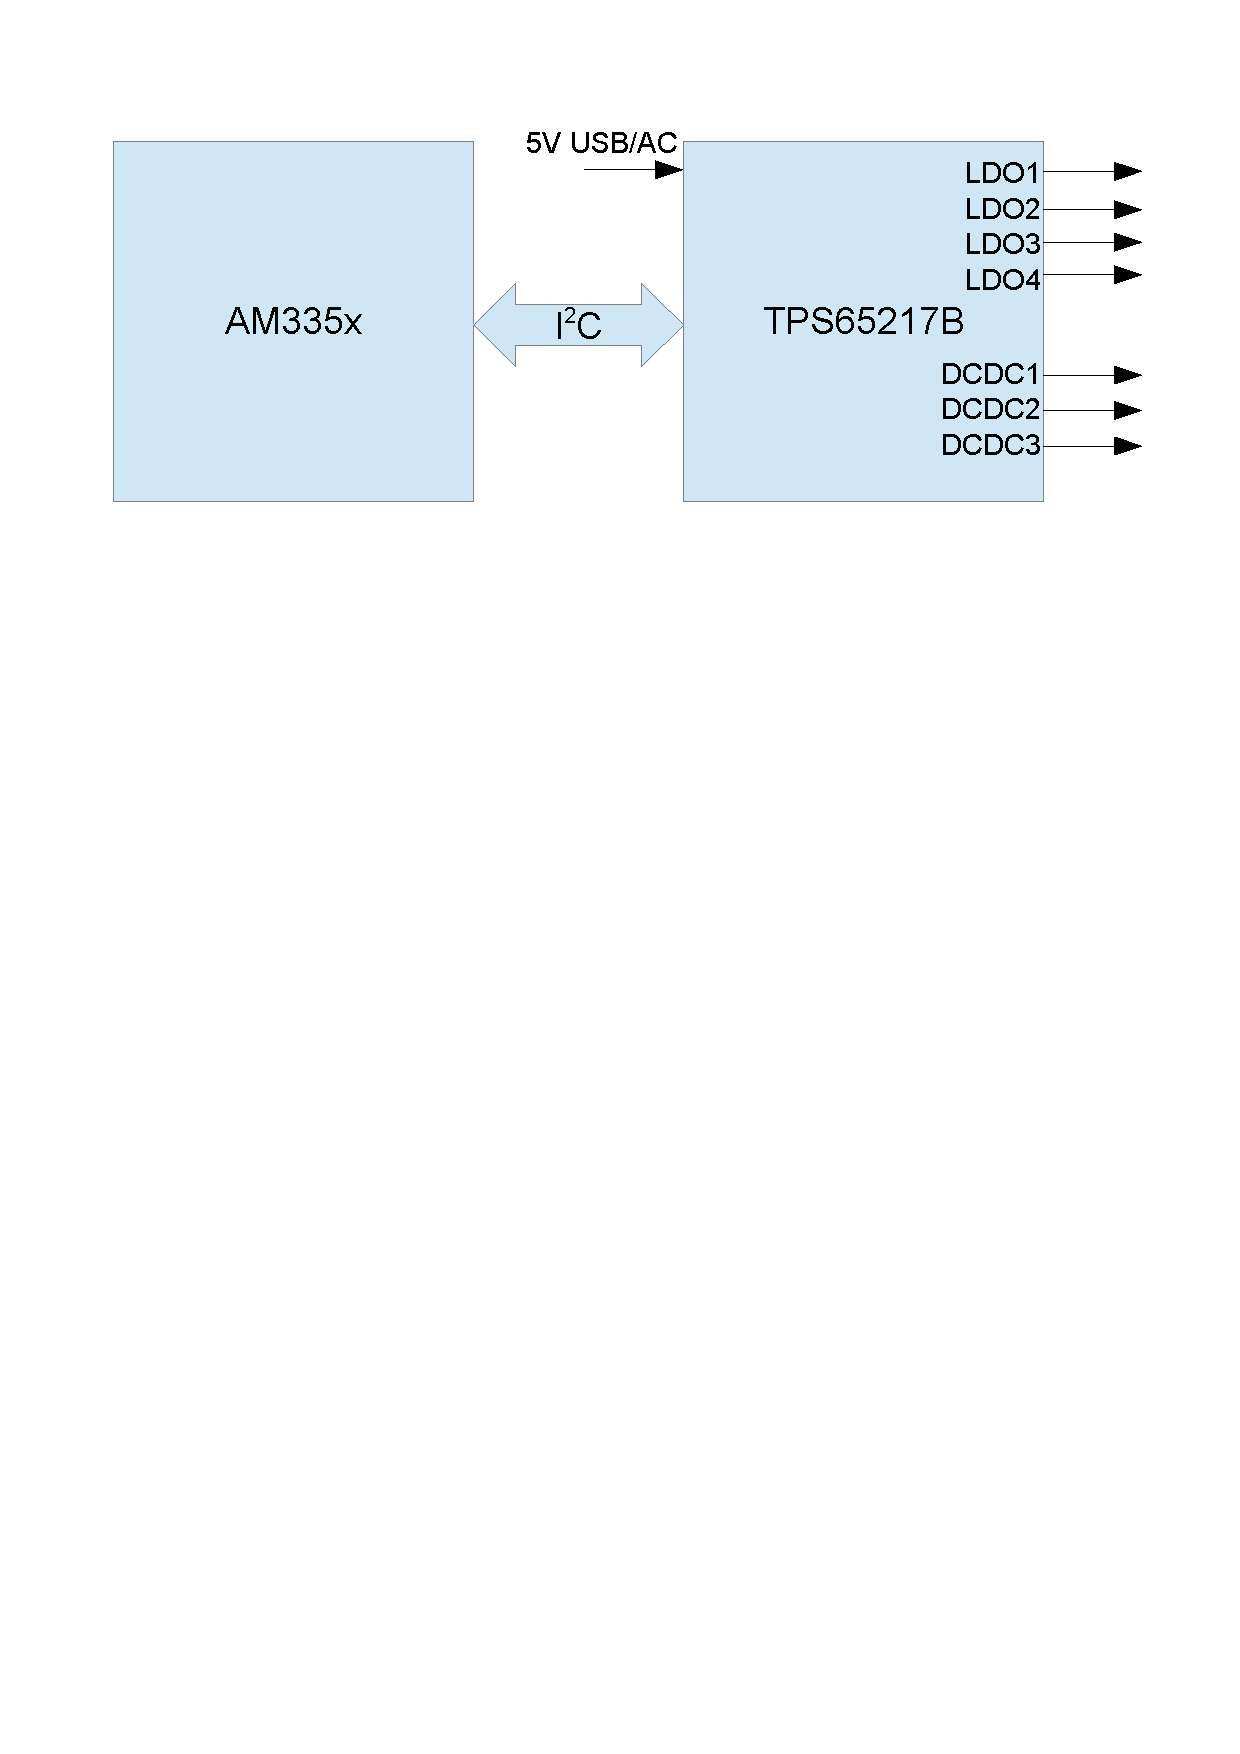
\includegraphics[width=300pt]{img_am335x-tps65217.pdf}
\end{frame}


\begin{frame}
\frametitle{Architektura naszej aplikacji wbudowanej}
\begin{center}
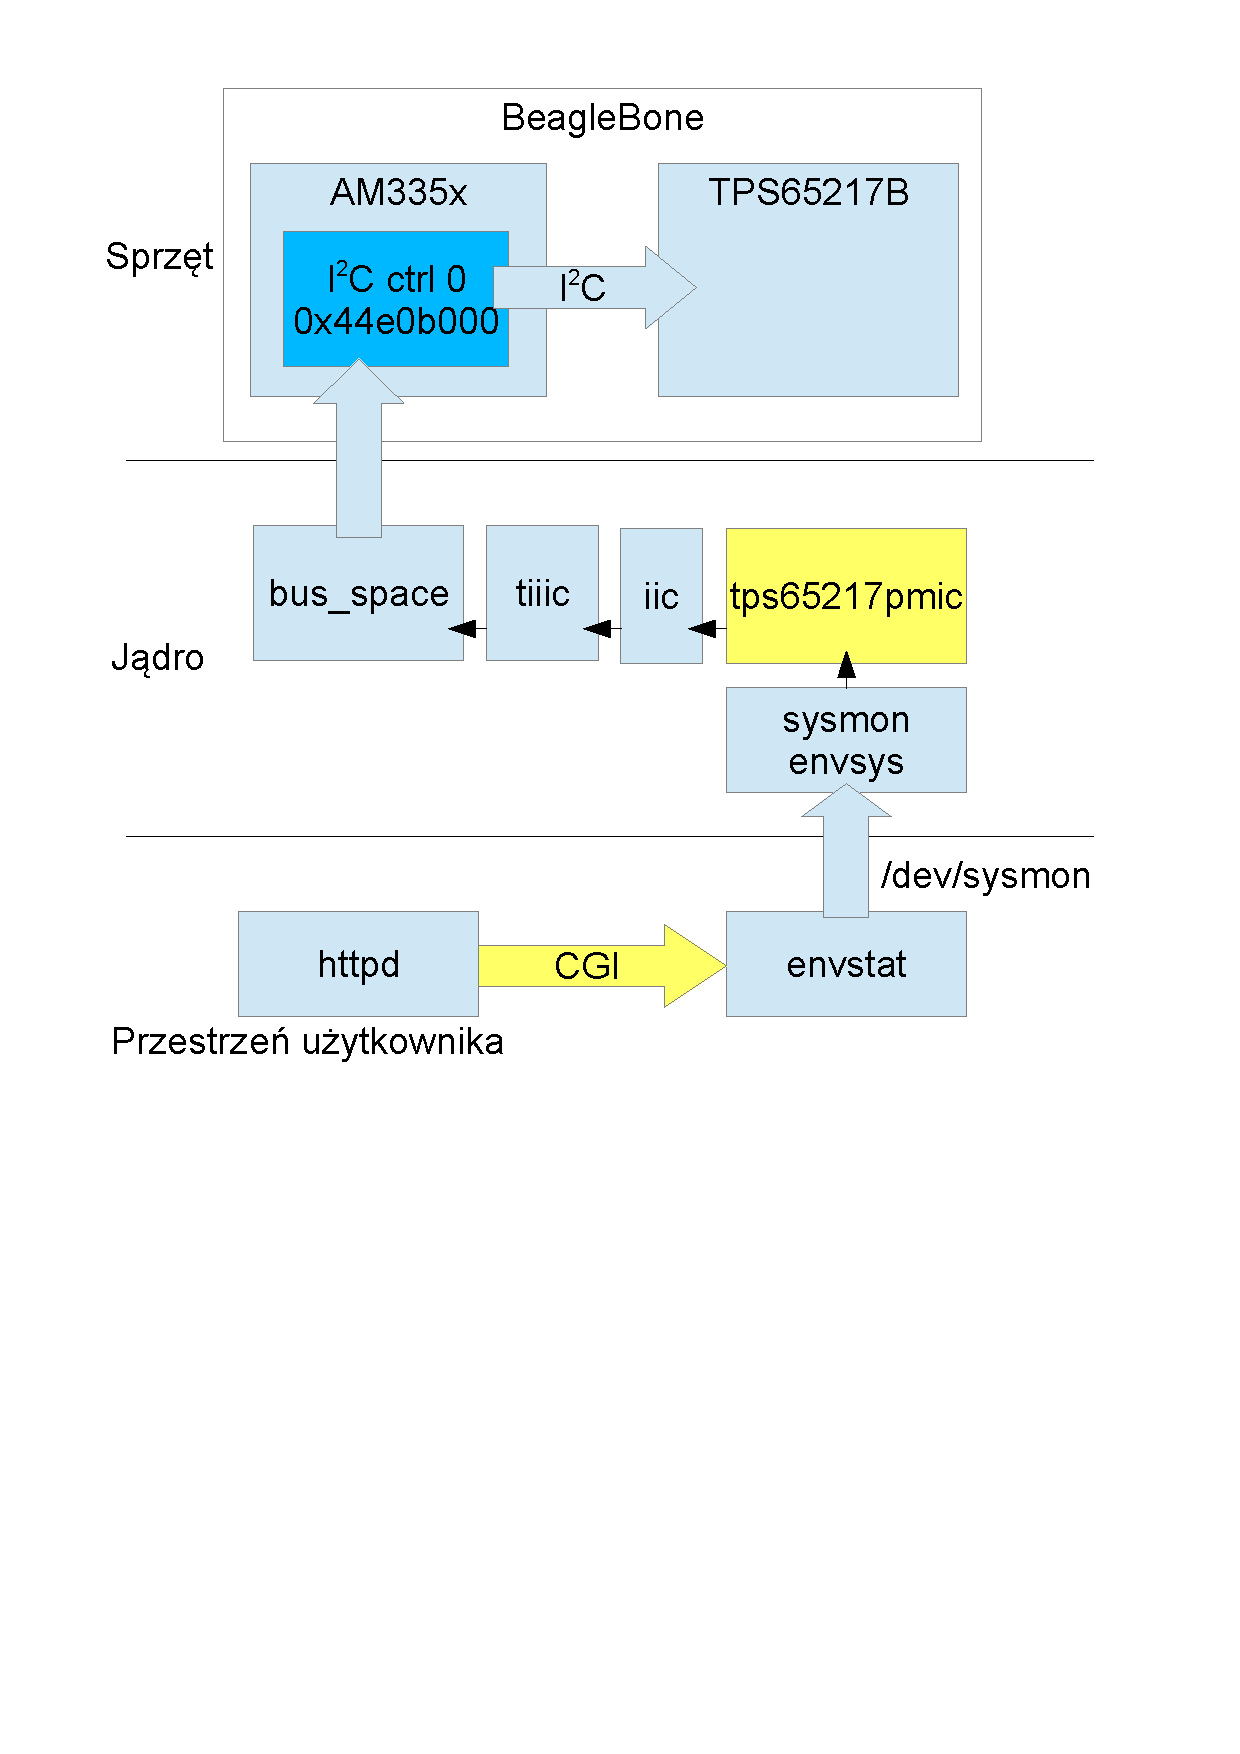
\includegraphics[scale=0.42]{img_apparch.pdf}
\end{center}
\end{frame}


\begin{frame}
\frametitle{Sterownik układu TPS65217B}
\begin{itemize}
	\item Sterownik \href{http://netbsd.gw.com/cgi-bin/man-cgi?tps65217pmic+4+NetBSD-current}{tps65217pmic(4)}
	\item Źródła
	\begin{itemize}
		\item \href{http://nxr.netbsd.org/xref/src/sys/dev/i2c/tps65217pmic.c}{src/sys/dev/i2c/tps65217pmic.c}
		\item \href{http://nxr.netbsd.org/xref/src/sys/dev/i2c/tps65217pmicreg.h}{src/sys/dev/i2c/tps65217pmicreg.h}
		\item Rejestracja istnienia sterownika w \href{http://nxr.netbsd.org/xref/src/sys/dev/i2c/files.i2c}{files.i2c}
	\end{itemize}
	\item Wykorzystuje niezależny od platformy sterownik szyny I\textsuperscript{2}C - \href{http://netbsd.gw.com/cgi-bin/man-cgi?iic+9+NetBSD-current}{iic(4)}
	\item Wykorzystuje interfejs \href{http://netbsd.gw.com/cgi-bin/man-cgi?sysmon_envsys+9+NetBSD-current}{sysmon\_envsys(4)} do przekazywania danych do przestrzeni użytkownika
	\item Konfiguracja jądra
	\begin{itemize}
		\item \href{http://nxr.netbsd.org/xref/src/sys/arch/evbarm/conf/BEAGLEBONE}{src/sys/arch/evbarm/conf/BEAGLEBONE}
		\item tps65217pmic*	at iic0 addr 0x24
	\end{itemize}
	\item Test z powłoki
	\begin{itemize}
		\item Polecenie \href{http://netbsd.gw.com/cgi-bin/man-cgi?envstat+8+NetBSD-current}{envstat(8)}
	\end{itemize}
\end{itemize}
\end{frame}

\defverbatim[colored]\lstCGI{%
\begin{lstlisting}
#!/bin/sh
REGULATORS="LDO1 LDO2 LDO3 LDO4 DCDC1 DCDC2 DCDC3"
echo "Content-type: text/html"
echo
echo "<html><body>"
for i in $REGULATORS
do 
	/usr/sbin/envstat | grep "^.*$i" | awk '{ print $2 }'
	echo <br/>
done
echo "</body></html>"
\end{lstlisting}
}

\begin{frame}[fragile]
\frametitle{Serwer HTTP jako interfejs użytkownika}
\begin{itemize}
	\item NetBSD posiada wbudowany daemon \href{http://netbsd.gw.com/cgi-bin/man-cgi?httpd++NetBSD-current}{httpd(8)}
	\item Obsługa CGI (oraz języków skryptowych jak PHP, Python)	
	\item Najprostsze rozwiązanie dla aplikacji wbudowanej:
	\begin{itemize}
		\item Skrypt powłoki wykonywany przez serwer HTTP
		\item Uruchamia polecenia systemowe
		\item Przedstawia wynik w formie HTML
	\end{itemize}
	\item Konfiguracja i uruchomienie:
	\begin{itemize}
		\item /etc/rc.conf: httpd=YES httpd\_flags="-c /var/cgi/"
		\item /etc/rc.d/httpd start
		\item Skopiowanie skryptu do katalogu /var/cgi/
	\end{itemize}

\end{itemize}
\lstCGI
\end{frame}

\begin{frame}
\frametitle{To działa!}
\begin{itemize}
	\item Skieruj przeglądarkę na adres http://adres\_beaglebone/cgi-bin/voltages.cgi
	\item Proste dzięki wykorzystaniu technik i narzędzi znanych z systemów serwerowych
\end{itemize}
\end{frame}

\begin{frame}
\frametitle{Co można zrobić dalej w tej aplikacji?}
\begin{itemize}
	\item Wyświetlanie napięć na zewnętrznym LCD (tekstowym lub graficznym)
	\item Przełączanie widoku na LCD za pomocą przycisków
	\item Przechowywanie i wyświetlanie danych historycznych
	\item Monitoring rzeczywistego napięcia na wyjściach
	\begin{itemize}
		\item Wykorzystanie wyjścia MUX\_OUT
		\item Konwersja A/C w AM335x (linia A7)
	\end{itemize}
	\item Możliwość rekonfiguracji regulatorów w trakcie pracy
	\item Obsługa zasilania bateryjnego (ładowanie, monitoring stanu baterii)
	\item Obsługa przerwań (linia NNMI)
\end{itemize}
\end{frame}

\begin{frame}
\frametitle{Propozycje innych prostych systemów wbudowanych}
\begin{itemize}
	\item Do zrealizowania z użyciem BealgeBone oraz dodatkowych modułów
	\begin{itemize}
		\item Stacja pogody (np. czujniki MPL115A2, MCP9801, wyświetlacz LCD)
		\item Odtwarzacz audio (np. przetwornik TS4657, wyświetlacz LCD, przyciski)
		\item foo
		\item bar
	\end{itemize}
\end{itemize}
\end{frame}


\section{Podsumowanie}

\begin{frame}
\frametitle{Podsuowanie}
\begin{itemize}
	\item NetBSD w zastosowaniach wbudowanych sprawdza się... etc.
	\item Potwierdza to wykorzystanie komercyjne przez czołowe firmy informatyczne
\end{itemize}
\end{frame}


\begin{frame}
\frametitle{Jeśli system NetBSD was zainteresował...}
\begin{columns}[c]
\column{3in}

\begin{itemize}
	\item \href{http://www.NetBSD.org/}{Oficjalna strona NetBSD }
	\item \href{http://www.netbsd.org/docs/guide/en/}{The NetBSD Guide}
	\item \href{http://www.embeddedarm.com/software/arm-netbsd-toaster.php}{NetBSD based toaster}
	\item \href{http://misc.allbsd.de/Vortrag/EuroBSDCon_2007/Stephen_Borrill/eurobsdcon.pdf}{Building products with NetBSD - thin clients}
	\item Kontakt do mnie
	\begin{itemize}
		\item rkujawa@NetBSD.org
		\item \href{http://wiki.NetBSD.org/users/rkujawa}{wiki.NetBSD.org/users/rkujawa}
	\end{itemize}
\end{itemize}

\column{1.5in}
	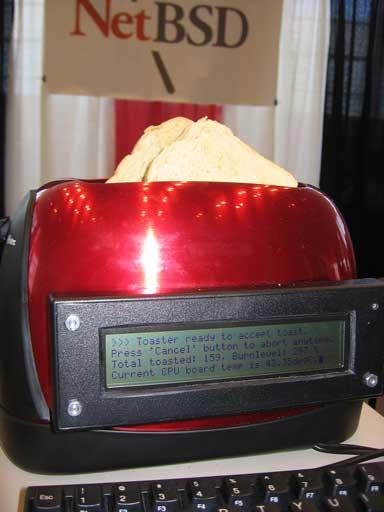
\includegraphics[scale=0.4]{img_netbsdtoaster.jpg}
\end{columns}

\end{frame}

\begin{frame}
\frametitle{Pytania}
\begin{itemize}
	\item Czy są jakieś pytania?
\end{itemize}
\end{frame}

\begin{frame}
\frametitle{Koniec\ldots}
\vspace*{-0.8cm}
\begin{center}

\includegraphics[scale=0.5]{NetBSD.png}

Dziękuje!
\end{center}
\end{frame}

 
\end{document}
